\documentclass[11pt,a4paper]{article}

\usepackage[utf8]{inputenc}
\usepackage[T1]{fontenc}
\usepackage[spanish]{babel}
\usepackage[margin=2.5cm]{geometry}
\usepackage{graphicx}
\usepackage{booktabs}
\usepackage{caption}
\usepackage{float}
\usepackage{hyperref}
\usepackage{amsmath}
\usepackage{amssymb}

\graphicspath{{figures/}}

\title{Documentación de gráficos --- TP5 Kuramoto (Sistema 1)}
\author{}
\date{}

\begin{document}
\maketitle

Este documento describe cada gráfico generado para el oscilador de Kuramoto:
qué representa cada eje, por qué se eligieron los rangos de barrido, y por qué
cada figura se ve como se ve. Las figuras son las mismas que aparecen en la
presentación.

\section{Parámetros comunes a todas las simulaciones}

Valores compartidos por los tres barridos (ver \texttt{run\_complete.py},
\texttt{run\_random.py}, \texttt{run\_ring.py}):

\begin{itemize}
  \item $N = 600$ osciladores.
  \item Frecuencias naturales gaussianas: $\omega_i \sim \mathcal{N}(\mu_\omega=1{,}0,\ \sigma_\omega=0{,}1)$.
  \item Fases iniciales uniformes: $\theta_i(0) \sim \mathcal{U}[0, 2\pi)$.
  \item $dt = 10^{-3}$ (paso de integración, RK4).
\end{itemize}

Lo que \emph{cambia} entre topologías:

\begin{table}[H]
  \centering
  \begin{tabular}{lccc}
    \toprule
    \textbf{Topología} & \textbf{Realizaciones (seeds)} & $t_{\text{sim}}$ & \textbf{Barrido} \\
    \midrule
    Completa  & 12 (\texttt{1000--1011}) & 50 s   & $K$ \\
    Aleatoria & 12 (\texttt{1000--1011}) & 100 s  & $p$, $K$ \\
    Anillo    & 50 (\texttt{1000--1049}) & 1500 s & $v$, $K$ \\
    \bottomrule
  \end{tabular}
  \caption{Diferencias por topología. Las curvas son promedios sobre las
  realizaciones y las barras de error son la desviación estándar entre ellas.
  El anillo usa 50 seeds (en vez de 12) por su alta dispersión realización a
  realización; ver la sección del anillo.}
\end{table}

\section{Observables}

\paragraph{Parámetro de orden $r(t)$.}
Mide la alineación instantánea de las fases:
\[
  r(t) = \left| \frac{1}{N} \sum_j e^{\,i\theta_j(t)} \right|
       = \left| \frac{1}{N} \sum_j [\cos\theta_j,\ \sin\theta_j] \right|.
\]
$r=0$ corresponde a fases repartidas uniformemente (desorden) y $r=1$ a todas
las fases iguales (sincronización global). Con $N$ finito, el estado
desordenado no da exactamente $0$ sino un piso $\sim 1/\sqrt{N} \approx 0{,}04$
(suma de $N$ vectores unitarios al azar; ver red completa, $K=0$).

\paragraph{Tiempo de sincronización $\tau$ (llegada al estado estacionario).}
Es el \emph{tiempo de establecimiento} (settling time): el primer instante a
partir del cual $r(t)$ deja de variar y se mantiene dentro de una banda de
$\pm 0{,}02$,
\[
  \tau = \min\Big\{\, t \ :\ \max_{s \ge t} r(s) - \min_{s \ge t} r(s) \le 0{,}04 \,\Big\}.
\]
A diferencia de un corte fijo, la ventana se adapta al transitorio real de cada
corrida. Se calcula sobre $r(t)$ suavizada con media móvil (banda $\pm 0{,}02$
del valor de régimen). El $0{,}02$ es la convención del 2\,\% del settling time,
aplicable porque $r \in [0,1]$.

\paragraph{Valor estacionario $r_\infty$.}
Es el promedio de $r(t)$ sobre la ventana ya establecida $[\tau, t_f]$,
\[
  r_\infty = \frac{1}{M} \sum_{t_k \ge \tau} r(t_k),
\]
donde $M$ es la cantidad de muestras con $t_k \ge \tau$. Es una suma discreta
(no una integral), fiel a lo que calcula el código (\texttt{np.mean}). Notar que
$\tau$ se define a partir del comportamiento de $r$ (cuándo se aplana) y
$r_\infty$ se promedia desde $\tau$: la dependencia es en una sola dirección,
no circular.

\section{Acoplamiento crítico $K_c$}

\subsection*{Criterio operativo (el que se marca en los gráficos)}

En la curva $r_\infty(K)$ de la red completa se define $K_c$ como el menor
acoplamiento para el cual el sistema queda \emph{más cerca de la sincronización
($r=1$) que del desorden ($r=0$)}, es decir $r_\infty \ge \tfrac{1}{2}$:
\[
  \boxed{\,K_c = \min\{\, K : r_\infty(K) \ge \tfrac{1}{2} \,\}\,}.
\]
El cruce se interpola en escala $\log K$ entre los dos puntos del barrido que lo
encierran. Para la red completa da $K_c \approx 3{,}7\cdot 10^{-4}$.

\subsection*{Referencia teórica (campo medio)}

La ecuación que integra el motor es
\[
  \frac{d\theta_i}{dt} = \omega_i + K \sum_{j \in \mathcal{N}(i)} \sin(\theta_j - \theta_i),
\]
donde $K$ multiplica directamente la suma sobre vecinos (sin dividir por $N$ ni
por el grado). El análisis de campo medio predice el \emph{inicio} de la
sincronización (onset) cuando el empuje promedio $K\langle k\rangle$ supera un
umbral, con $\langle k\rangle$ el grado medio:
\[
  K_c^{\text{MF}} = \frac{\sigma\,\sqrt{8/\pi}}{\langle k\rangle}.
\]
Con $\sigma = 0{,}1$, $K_c^{\text{MF}} \approx 0{,}16/\langle k\rangle$. Para la
red completa ($\langle k\rangle = 599$) da $\approx 2{,}7\cdot 10^{-4}$. El $K_c$
operativo ($r_\infty = \tfrac12$, $\approx 3{,}7\cdot 10^{-4}$) cae algo por
encima del teórico porque $r = 0{,}5$ se alcanza un poco después de la
emergencia. \textbf{$K_c^{\text{MF}}$ depende de la topología} vía $\langle k\rangle$:

\begin{table}[H]
  \centering
  \begin{tabular}{lcc}
    \toprule
    \textbf{Topología} & $\langle k \rangle$ con $N=600$ & $K_c^{\text{MF}}$ \\
    \midrule
    Completa            & 599        & $\sim 2{,}7\cdot 10^{-4}$ \\
    Aleatoria $p=0{,}1$ & $\sim 60$  & $\sim 2{,}7\cdot 10^{-3}$ \\
    Aleatoria $p=0{,}01$& $\sim 6$   & $\sim 0{,}03$ \\
    Aleatoria $p=10^{-4}$& $\sim 0{,}06$ & (red fragmentada) \\
    Anillo $v=10$       & 20         & $\sim 8\cdot 10^{-3}$ \\
    Anillo $v=1$        & 2          & $\sim 0{,}08$ \\
    \bottomrule
  \end{tabular}
  \caption{$K_c$ teórico (onset) por topología.}
\end{table}

\subsection*{Efectos topológicos más allá de $K_c$}

Superar $K_c$ es \textbf{necesario pero no suficiente} para sincronizar
globalmente:
\begin{itemize}
  \item \textbf{Aleatoria con $p < p_c \approx \ln N / N \approx 0{,}011$}: la red
  está fragmentada (no hay componente gigante). Aunque $K \to \infty$, las fases
  de componentes desconectadas no pueden comunicarse y $r$ no llega a 1.
  \item \textbf{Anillo con $v$ chico}: aun siendo conexo, soporta \emph{estados
  twisted} (la fase da una o más vueltas a lo largo del anillo). Son mínimos
  locales estables donde el sistema queda atrapado mucho tiempo. Además la
  información se propaga sólo entre vecinos cercanos, así que los transitorios
  son enormes (de ahí $t_{\text{sim}} = 1500$).
\end{itemize}

\section{Por qué los mapas de calor tienen celdas sin pintar}

Hay dos tipos de mapa y se comportan distinto:

\begin{itemize}
  \item \textbf{Mapas de $r_\infty$} ($r_\infty(p,K)$, $r_\infty(v,K)$):
  \textbf{están completamente pintados}. $r_\infty$ siempre se puede calcular
  (es el promedio de $r$ en el régimen, exista o no sincronización): donde no
  sincroniza simplemente vale poco (color oscuro), no queda en blanco.

  \item \textbf{Mapas de $\tau$} ($\tau(p,K)$, $\tau(v,K)$): \textbf{tienen celdas
  blancas}. La consigna pide el ``tiempo de sincronización \emph{o llegada al
  estado estacionario}''. $\tau$ es ese tiempo: el transitorio desde el desorden
  inicial hasta el estado estacionario \emph{ordenado}. Una celda se pinta si el
  sistema desarrolla orden --- al menos el 25\% de las realizaciones alcanza
  $r_\infty > 0{,}2$ (claramente por encima del piso $1/\sqrt N \approx 0{,}04$;
  $\ge 3$ realizaciones en completa/aleatoria con 12 seeds, $\ge 13$ en el anillo
  con 50); si no, queda en blanco.
\end{itemize}

\paragraph{El blanco $=$ ``se quedó desordenado'', y no es lo mismo en los dos mapas.}
Una celda blanca del mapa de $\tau$ \emph{no} está blanca en el de $r_\infty$: ahí
$r_\infty$ está pintado \textbf{oscuro} (el sistema se quedó en el piso
desordenado, $r \approx 0{,}04$). O sea: blanco-en-$\tau$ $\Leftrightarrow$
oscuro-en-$r_\infty$, nunca blanco-en-$r_\infty$ (ese mapa no tiene blancos). La
clave: en esas celdas \textbf{no hay transitorio que medir}. El sistema arranca
con fases al azar ($r \approx 1/\sqrt N$) y se queda ahí --- ya está en su estado
estacionario desde $t \approx 0$ ---, así que su tiempo de llegada al estacionario
es trivialmente $\sim 0$, no un valor grande.

\paragraph{$\tau$ existe pero no se grafica ahí.}
El algoritmo devuelve un $\tau$ (settling time) para cualquier corrida, pero en las
celdas desordenadas ese número es \emph{espurio}: en la aleatoria fragmentada el
detector de banda pelea con el ruido del piso y da $\tau \sim 70$--$80$ s, y en el
anillo que driftea $\tau$ choca contra el tope de la ventana
($\approx t_{\text{sim}}$, $\sim 1400$ s). Ninguno es un transitorio real (no hubo
transitorio). Si los pintáramos, la región desordenada aparecería \emph{más lenta}
que la ordenada, sugiriendo falsamente ``tarda muchísimo en ordenarse'' cuando en
realidad nunca se ordena. Por eso se filtran.

\paragraph{Por qué el umbral es $r_\infty > 0{,}2$ y no $> 0{,}5$.}
Se usa $0{,}2$ para \textbf{incluir los estados parcialmente ordenados}: hay celdas
--- sobre todo en el anillo --- donde $r$ se asienta en un valor intermedio
(p.\,ej.\ $0{,}3$) con un transitorio real, un ``llegada al estacionario''
genuino. Con $r_\infty > 0{,}5$ las ocultábamos; con $0{,}2$ (claramente por encima
del piso $\sim 0{,}04$) se muestran. Es un umbral distinto al del $K_c$
($r_\infty \ge \tfrac12$), que no se toca.

\paragraph{Por qué 50 seeds en el anillo.}
Cerca de la transición el resultado es ruidoso: según la condición inicial, una
realización desarrolla orden o queda atrapada en un estado twisted. El criterio de
``$\ge 25\%$ desarrolla orden'' con sólo 12 seeds (o sea $\ge 3$) descansa en muy
pocas corridas y es inestable. Con 50 seeds ese mismo 25\% pasa a ser $\ge 13$
realizaciones: el conteo es mucho más confiable, cada celda pintada se apoya en
$\ge 13$ corridas y las medias y barras de error quedan bien estimadas.

\section{Por qué escala logarítmica en $K$, $p$ y $\tau$}

El barrido de esos parámetros cubre varios órdenes de magnitud; en escala lineal
los puntos chicos quedarían aplastados contra el origen. Por ejemplo, $K$ va de
$10^{-4}$ a $1$ (4 órdenes): en lineal, $0{,}0001$, $0{,}001$, $0{,}01$ son
indistinguibles de cero frente a $1$, y la transición se ve como un único salto
sin estructura. En log cada orden de magnitud ocupa el mismo ancho, los puntos
quedan equiespaciados y se ve la forma real de la transición. Hay además un
motivo físico: cuando no se conoce a priori el valor crítico, lo natural es
muestrear logarítmicamente, y el gráfico respeta cómo fue diseñado el barrido.

\begin{itemize}
  \item $K$ y $p$ en log (barridos sobre 3--4 órdenes de magnitud).
  \item $\tau$ en log \emph{sólo} en la comparativa entre topologías, porque ahí
  difieren en órdenes de magnitud; dentro de una topología, $\tau$ va en lineal.
  \item $v$ (vecindad del anillo) en lineal: entero de 1 a 10, un solo orden.
  \item $r$ en lineal: está acotado a $[0, 1]$ por definición.
\end{itemize}

\subsection*{Por qué no se muestrea linealmente $K$ y $p$ en $[0,1]$}

El enunciado pide al menos 10 puntos. Un muestreo lineal $K = 0{,}1,\,0{,}2,
\ldots,\,1{,}0$ cumple la letra pero no muestra nada: el crítico de la completa
es $K_c \approx 2{,}7\cdot 10^{-4}$, así que esos 10 puntos quedan varios órdenes
por encima y todos dan $r \approx 1$. Para $p$, la física vive en
$p \sim 10^{-3}$--$10^{-2}$ (umbral de percolación $p_c \approx \ln N / N \approx
0{,}011$); un muestreo $p = 0{,}1, \ldots, 1{,}0$ dejaría todo conectado y el
gráfico sería una línea plana en $r \approx 1$. Por eso se muestrea log:
$p \in \{10^{-4}, 2\!\cdot\!10^{-4}, 5\!\cdot\!10^{-4}, 10^{-3}, 2\!\cdot\!10^{-3},
5\!\cdot\!10^{-3}, 0{,}01, 0{,}02, 0{,}05, 0{,}1\}$, con $p_c$ holgadamente
cubierto.

\section{Red totalmente conectada}

Barrido $K \in \{0, 10^{-4}, 3\!\cdot\!10^{-4}, 5\!\cdot\!10^{-4}, 10^{-3},
3\!\cdot\!10^{-3}, 0{,}01, 0{,}03, 0{,}1, 0{,}3, 1\}$ (cuasi-log, 4 órdenes),
más una grilla fina extra en la zona de transición ($1$--$6\cdot 10^{-4}$) para
resolver bien el cruce de $r_\infty$. Se incluye $K = 0$ como control (sin
acoplamiento, $r$ debe quedar en el piso $\sim 1/\sqrt N$). $t_{\text{sim}} = 50$
porque la red completa sincroniza en pocas unidades de tiempo.

\subsection{Evolución temporal $r(t)$}

\begin{figure}[H]
  \centering
  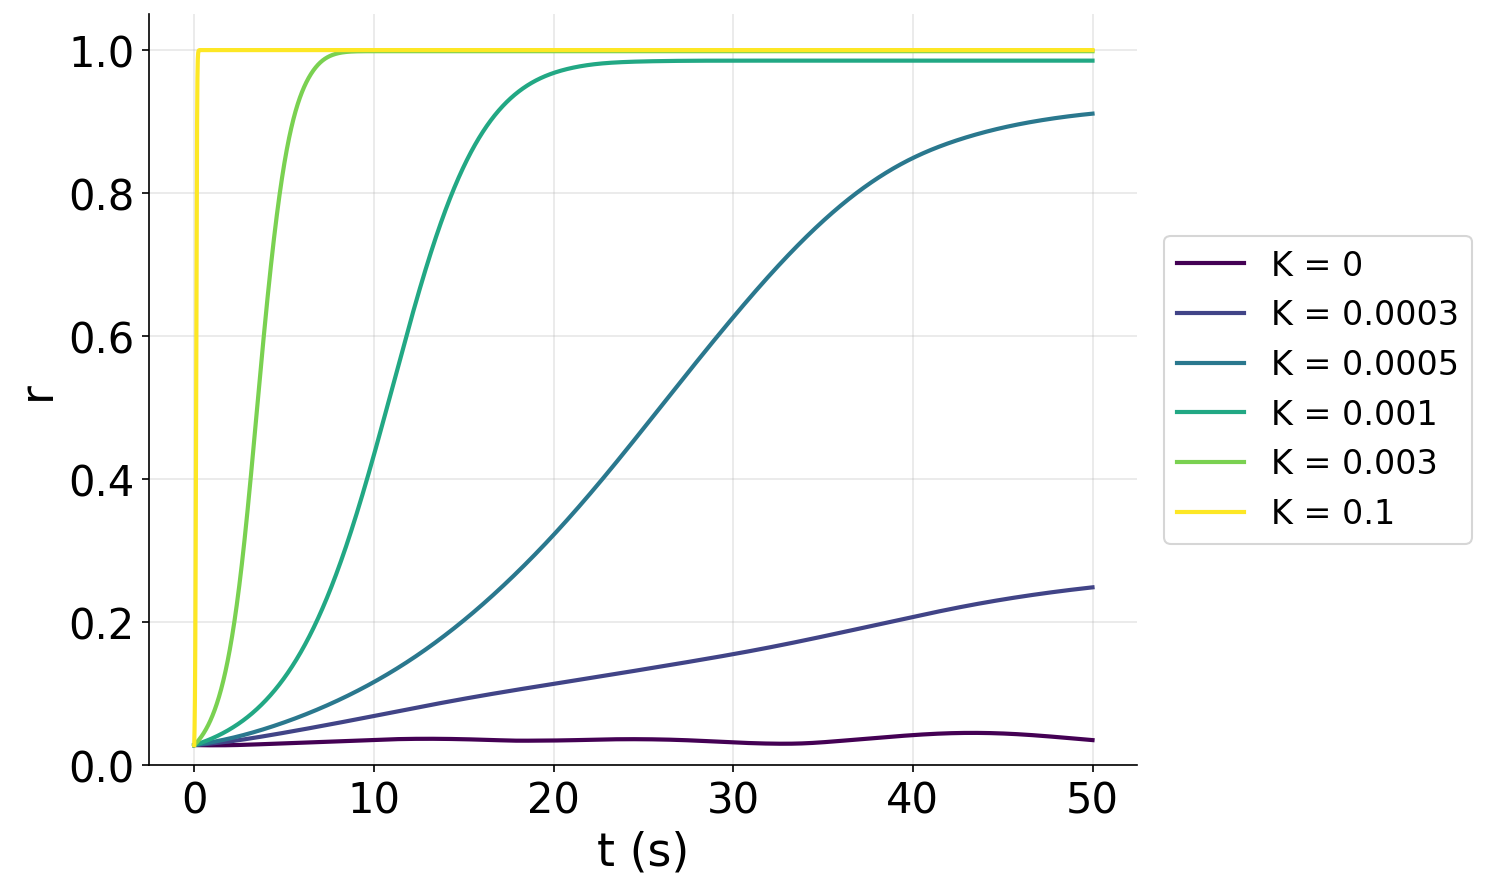
\includegraphics[width=0.8\linewidth]{complete_rt.png}
  \caption{$r(t)$ para un subconjunto representativo de $K$, promediado sobre 12 seeds.}
\end{figure}

\begin{itemize}
  \item \textbf{Eje X}: tiempo $t$ (s), de 0 a 50.
  \item \textbf{Eje Y}: parámetro de orden $r(t) \in [0,1]$.
  \item \textbf{Curvas}: una por cada $K$ mostrado (viridis: oscuro $=$ $K$ bajo,
  claro $=$ $K$ alto). Se muestran sólo \emph{6 valores representativos} porque
  los $K$ altos ($0{,}01$--$1$) dan curvas casi idénticas (suben a 1 al instante)
  y saturarían la leyenda; la leyenda va afuera del gráfico para no tapar las curvas.
\end{itemize}

Se ve la transición: para $K$ chico $r$ queda en el piso ($K=0$ fluctúa en
$\sim 0{,}04 = 1/\sqrt{600}$, no en 0, por el tamaño finito); al cruzar $K_c$
aparece la rama sincronizada y se estabiliza en un plateau cercano a 1. Cuanto
mayor $K$, más rápido sincroniza.

\subsection{Curva de bifurcación $r_\infty(K)$}

\begin{figure}[H]
  \centering
  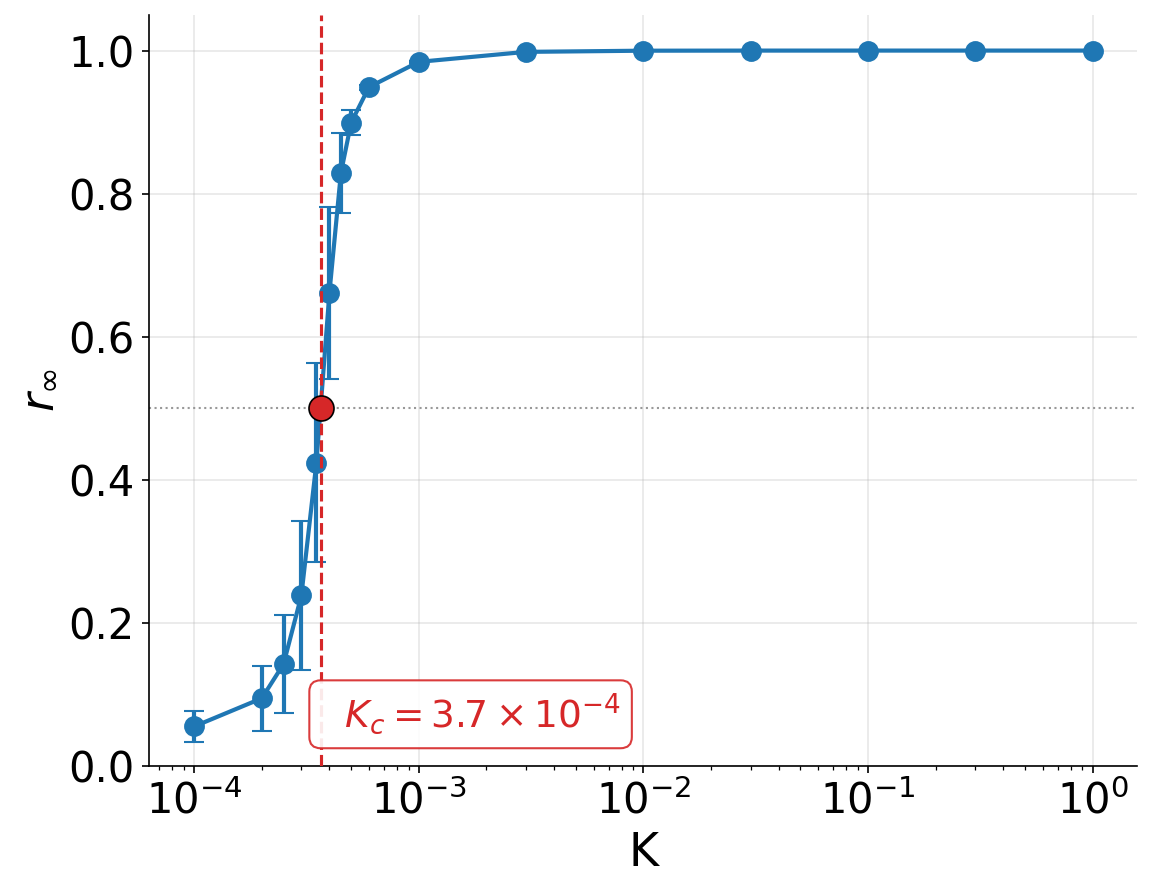
\includegraphics[width=0.7\linewidth]{complete_rK.png}
  \caption{Parámetro de orden estacionario vs $K$, con la marca de $K_c$.}
\end{figure}

\begin{itemize}
  \item \textbf{Eje X}: $K$ en escala \textbf{logarítmica} (barrido de 4 órdenes).
  \item \textbf{Eje Y}: $r_\infty(K)$ con barras de error (std entre seeds).
  \item \textbf{Marcas}: línea horizontal punteada en $r = 0{,}5$, línea vertical
  en $K_c$, y un punto rojo sobre la curva en el cruce. La etiqueta indica
  $K_c \approx 3{,}7\cdot 10^{-4}$.
\end{itemize}

Cerca del umbral la teoría predice $r_\infty(K) \approx \sqrt{(K-K_c)/K_c}$ (una
raíz cuadrada que arranca en $K_c$ y satura cerca de 1). Como el eje $K$ es
logarítmico, esa raíz se ve \textbf{comprimida en un salto abrupto}: los puntos a
la izquierda de la transición quedan pegados al piso y los de la derecha cerca de
1. La grilla fina en la zona de subida hace que el salto se vea bien resuelto.
El $K_c$ marcado es el cruce de $r_\infty = 0{,}5$ (criterio operativo). $K = 0$
se descarta del gráfico porque $\log 0 = -\infty$.

\subsection{Tiempo de sincronización $\tau(K)$}

\begin{figure}[H]
  \centering
  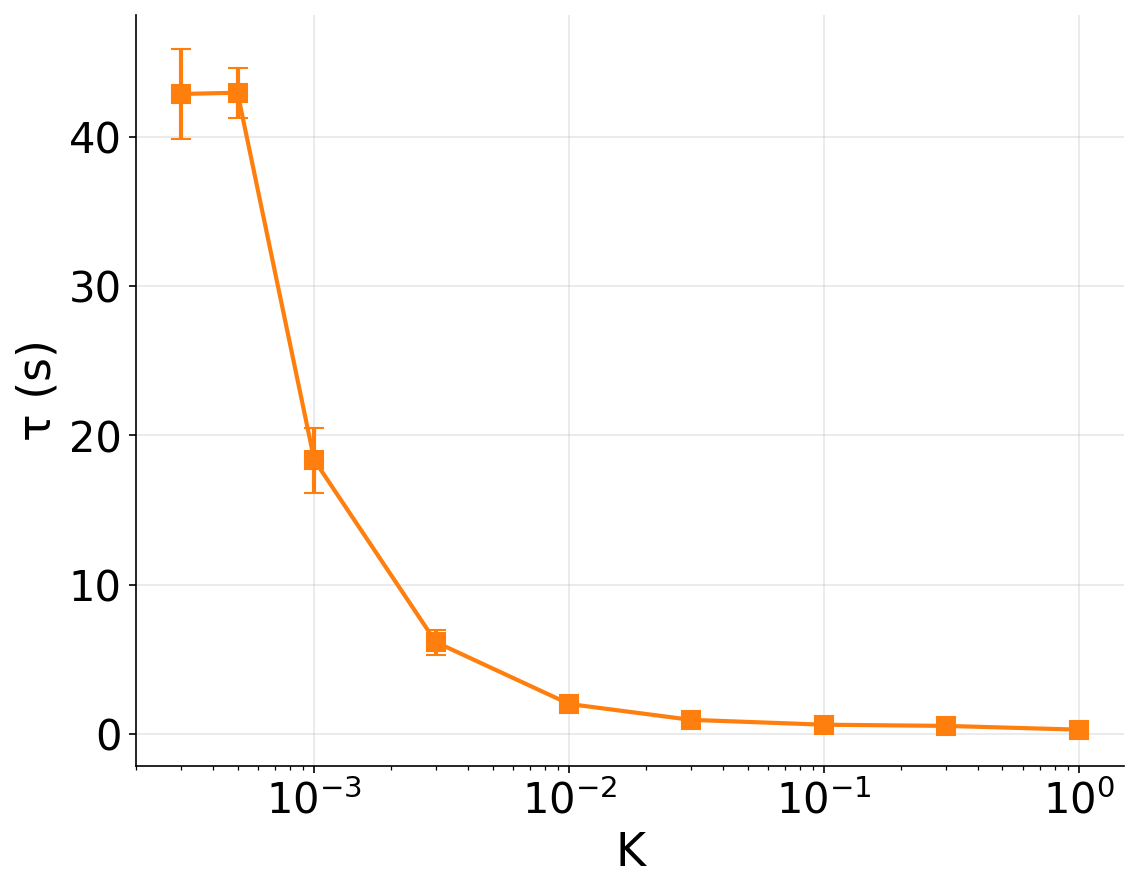
\includegraphics[width=0.7\linewidth]{complete_tauK.png}
  \caption{Tiempo de sincronización vs $K$.}
\end{figure}

\begin{itemize}
  \item \textbf{Eje X}: $K$ en log.
  \item \textbf{Eje Y}: $\tau$ (s), en lineal (rango moderado dentro de la topología).
\end{itemize}

Sólo se grafican los $K$ donde al menos el 25\% de las realizaciones (3 de 12) desarrolla orden ($r_\infty > 0{,}2$),
por eso hay menos puntos que en $r_\infty(K)$. $\tau$ \textbf{diverge cerca de
$K_c$} (\emph{critical slowing down}: justo en la transición el sistema tarda
muchísimo en ordenarse) y decae al aumentar $K$.

\section{Red aleatoria de Erd\H{o}s--Rényi}

Barridos: $p \in [10^{-4}, 10^{-1}]$ (10 valores log, rango del enunciado v2) y
$K \in \{10^{-3}, 3\!\cdot\!10^{-3}, 0{,}01, 0{,}03, 0{,}1, 0{,}3, 1\}$ (log). El
grado medio es $\langle k\rangle = p(N-1)$: desde $\sim 0{,}06$ en $p=10^{-4}$
(fragmentada) hasta $\sim 60$ en $p=0{,}1$ (bien conectada).

$t_{\text{sim}} = 100$ (la completa usa 50). Cuando la red tiene una componente
gigante densa su diámetro es chico ($\sim \ln N / \ln\langle k\rangle$) y
sincroniza tan rápido como la completa; el margen extra asegura que las pocas
corridas marginales cerca de la transición lleguen al estacionario. No hace falta
el $t_{\text{sim}}$ grande del anillo: donde la aleatoria sincroniza, lo hace
rápido; donde está fragmentada, no sincroniza por más tiempo que se le dé.

\subsection{Corte $r_\infty(p)$ a $K = 0{,}1$}

\begin{figure}[H]
  \centering
  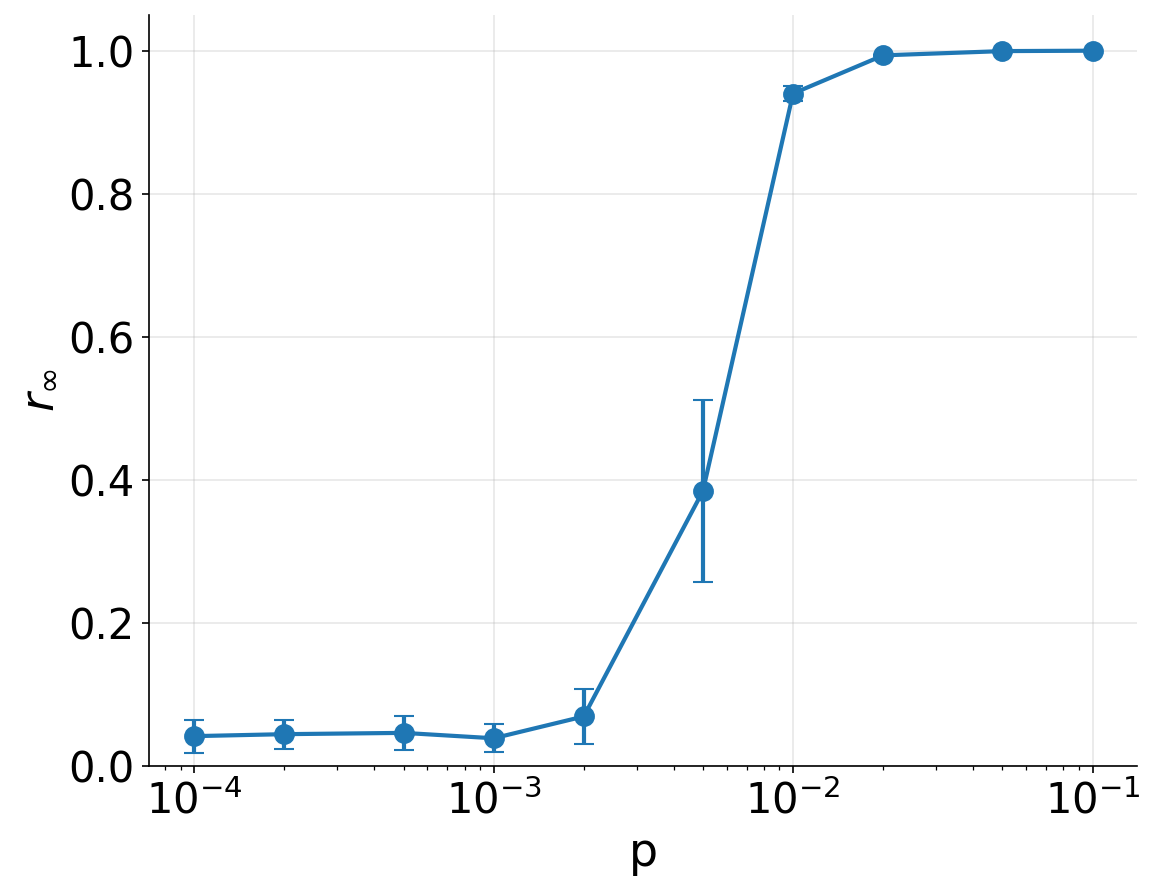
\includegraphics[width=0.7\linewidth]{random_rp.png}
  \caption{$r_\infty(p)$ fijando $K = 0{,}1$ (valor del enunciado v2).}
\end{figure}

\begin{itemize}
  \item \textbf{Eje X}: probabilidad de conexión $p$, en log.
  \item \textbf{Eje Y}: $r_\infty(p)$ con barras de error.
\end{itemize}

Fijado $K = 0{,}1$, la sincronización depende de la conectividad. Para
$p \lesssim 10^{-3}$ la red está fragmentada y $r$ queda en el piso
$\sim 1/\sqrt N$; la transición ocurre alrededor de $p \approx p_c \approx 0{,}011$
y, para $p \gtrsim 0{,}02$, ya hay componente gigante densa y $r \to 1$. A este
$K$ moderado el salto coincide con el \textbf{umbral de percolación} de
Erd\H{o}s--Rényi, no con el de acoplamiento.

\subsection{Mapa de calor $r_\infty(p, K)$}

\begin{figure}[H]
  \centering
  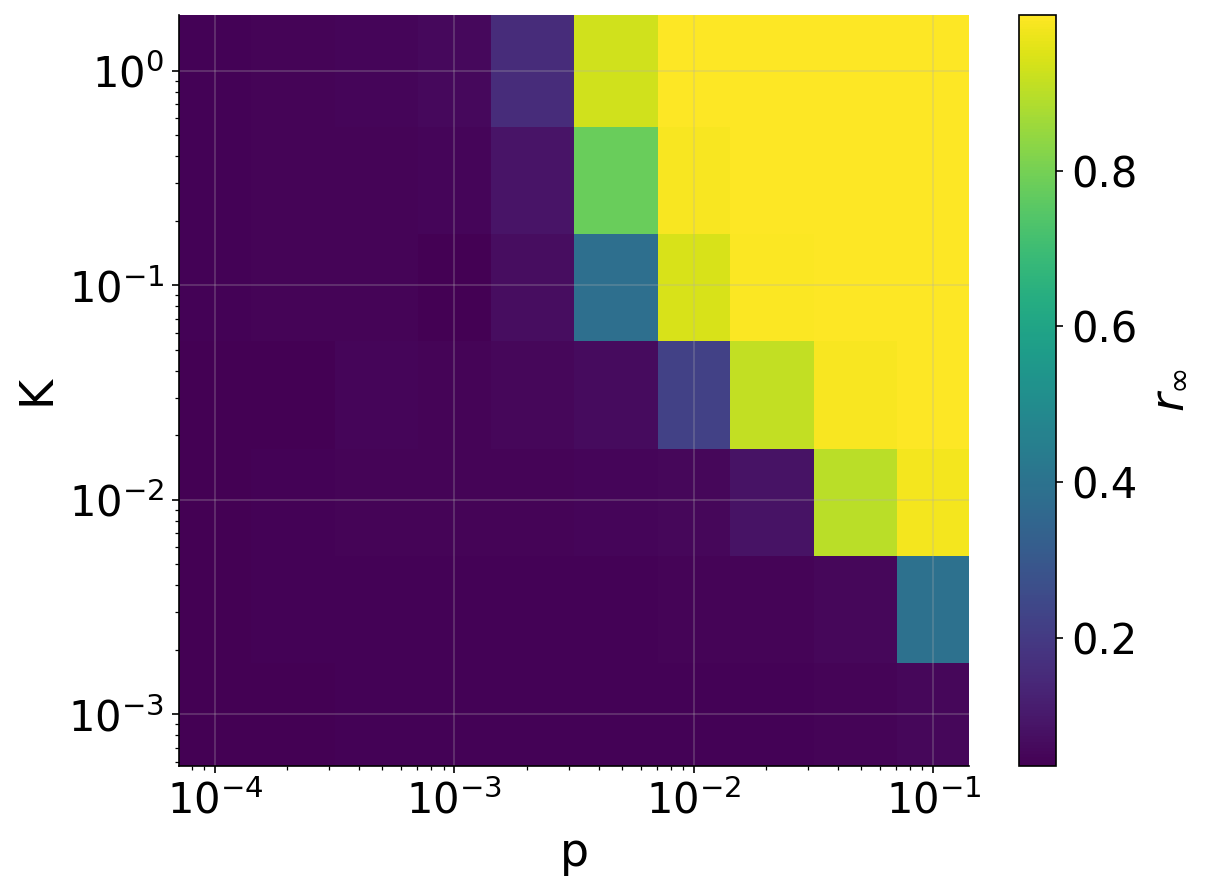
\includegraphics[width=0.8\linewidth]{random_rpK.png}
  \caption{Diagrama de fases en el plano $(p, K)$; color $= r_\infty$.}
\end{figure}

Ejes $p$ (log) y $K$ (log); color viridis ($0 \to 1$). La frontera diagonal
separa la región sincronizada (arriba-derecha, $K$ y $p$ altos) de la incoherente
(abajo-izquierda). \textbf{Sin celdas blancas}: $r_\infty$ siempre está definido.

\subsection{Mapa de calor $\tau(p, K)$}

\begin{figure}[H]
  \centering
  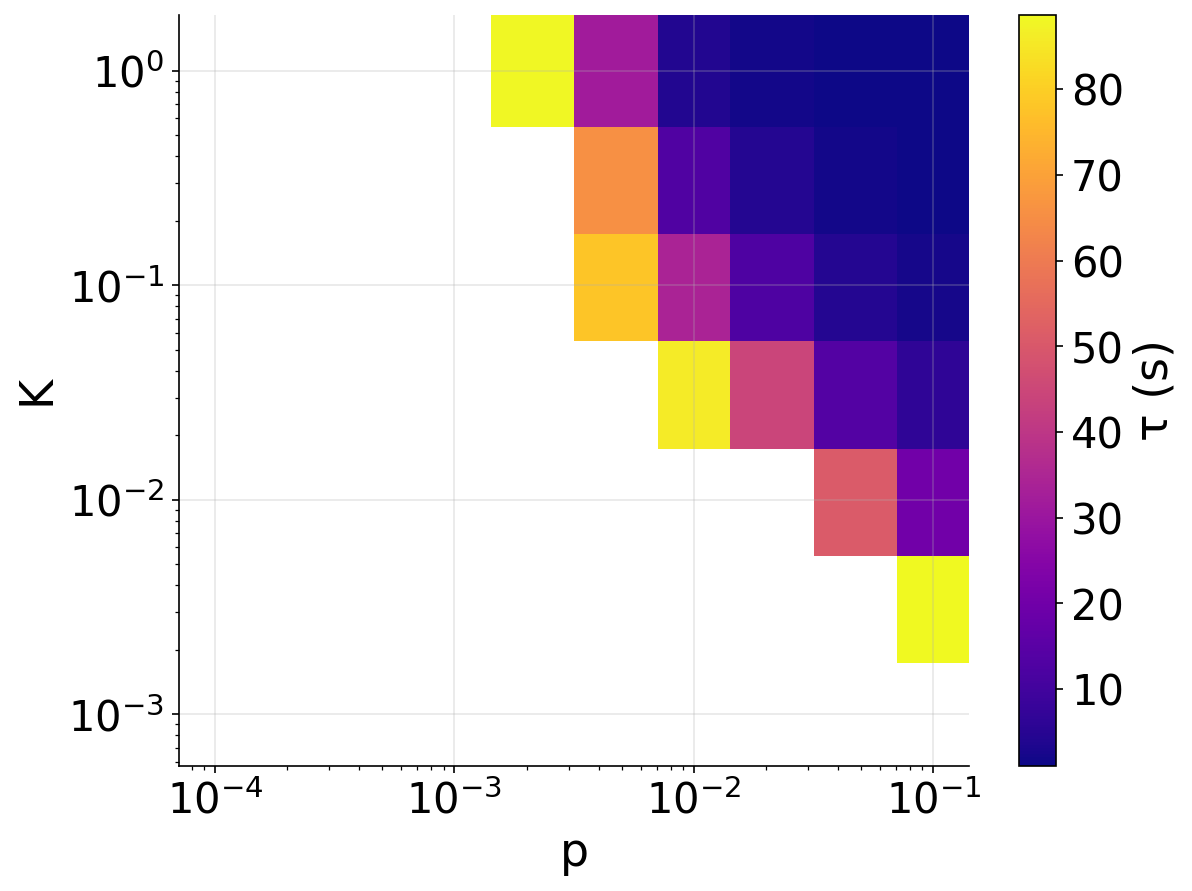
\includegraphics[width=0.8\linewidth]{random_taupK.png}
  \caption{Tiempo de sincronización en el plano $(p, K)$; color $= \tau$.}
\end{figure}

Mismo dominio; color plasma $= \tau$. Las \textbf{celdas blancas} son
combinaciones $(p, K)$ donde menos del 25\% de las realizaciones (3 de 12)
desarrolla orden ($r_\infty > 0{,}2$): la región fragmentada donde el sistema se
queda en el piso desordenado y no hay transitorio que cronometrar.

\section{Red en anillo con vecindad $v$}

Barridos: $v \in \{1, \ldots, 10\}$ (entero, lineal; cada nodo conecta a $v$
vecinos por lado, grado $2v$) y $K \in \{0{,}01, 0{,}03, 0{,}05, 0{,}1, 0{,}2,
0{,}3, 0{,}5, 1{,}0\}$ (log, más fina cerca de $K_c$).

$t_{\text{sim}} = 1500$ ($30\times$ más que las otras): el anillo tiene
transitorios larguísimos porque la información se propaga sólo a vecinos cercanos
(diámetro $\sim N/2v$, mucho mayor que el $\sim \ln N$ de la aleatoria conectada)
y los modos de fase tardan en homogeneizarse.

\paragraph{Por qué 50 seeds.} El anillo es la topología con mayor dispersión
realización a realización: cerca de la transición, según la condición inicial, el
sistema desarrolla orden o queda atrapado en un estado twisted. El criterio para
pintar una celda del mapa de $\tau$ es que desarrolle orden ($r_\infty > 0{,}2$) al
menos el 25\% de las realizaciones; con 12 seeds eso es $\ge 3$ corridas, un conteo
marginal e inestable. Con 50 seeds ese 25\% es $\ge 13$ corridas: el mapa queda
bien definido y las medias mucho más robustas (el error de la media baja como
$1/\sqrt{n}$). La dispersión \emph{en sí} no se achica --- es física --- pero se
mide mejor.

\subsection{Corte $r_\infty(v)$ a $K = 0{,}1$}

\begin{figure}[H]
  \centering
  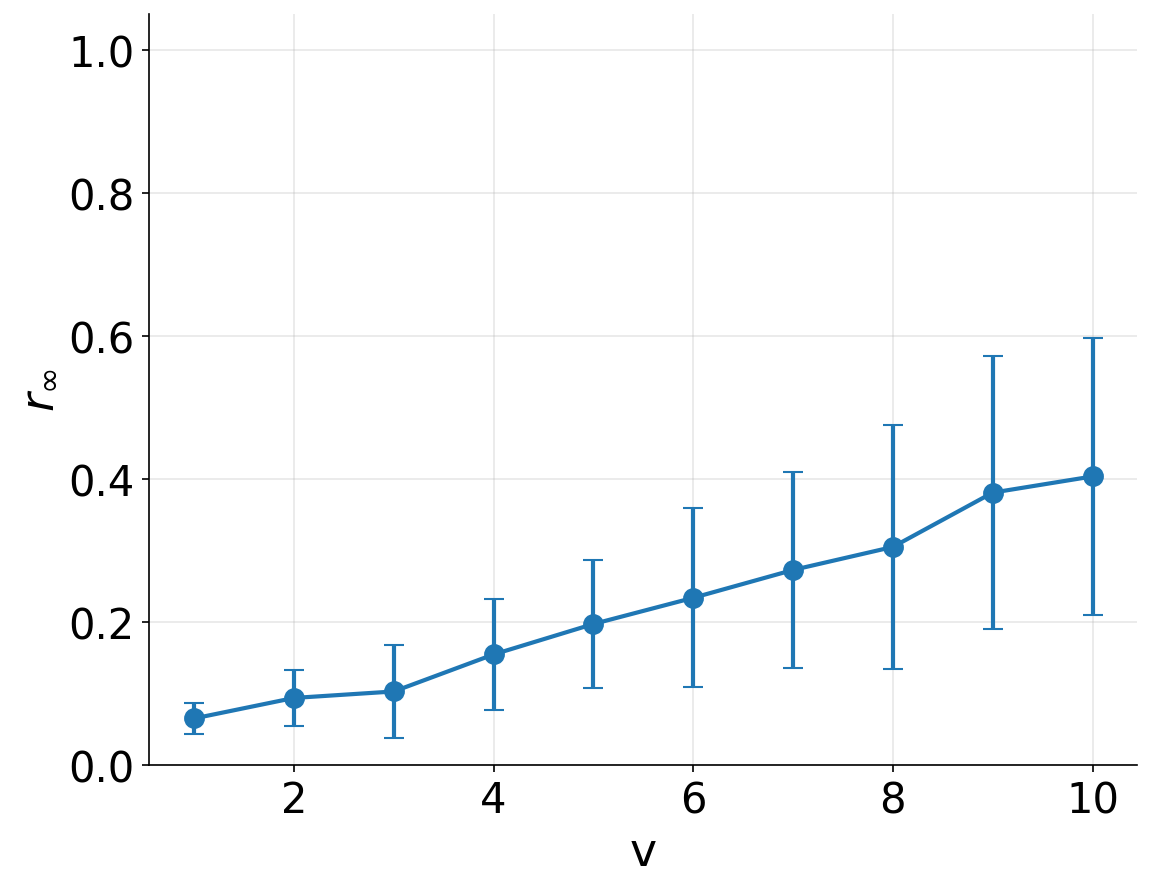
\includegraphics[width=0.7\linewidth]{ring_rv.png}
  \caption{$r_\infty(v)$ fijando $K = 0{,}1$ (valor del enunciado v2).}
\end{figure}

Ejes: $v$ (lineal, entero) y $r_\infty$ con barras de error. A $K = 0{,}1$,
$r_\infty$ crece de forma aproximadamente monótona con $v$ (de $\sim 0{,}06$ en
$v=1$ a $\sim 0{,}40$ en $v=10$) \textbf{sin saturar en 1}: a este acoplamiento
moderado, ni con $v=10$ alcanza la sincronización global. Con $v=1$ la red es casi
1D y sincronizar es muy difícil; al subir $v$ el grafo se acerca a la completa y
$r$ sube. Las \textbf{barras de error crecen con $v$} porque cerca de la
transición distintas realizaciones quedan en estados parcialmente sincronizados o
twisted diferentes (dispersión física, bien estimada con 50 seeds).

\subsection{Mapa de calor $r_\infty(v, K)$}

\begin{figure}[H]
  \centering
  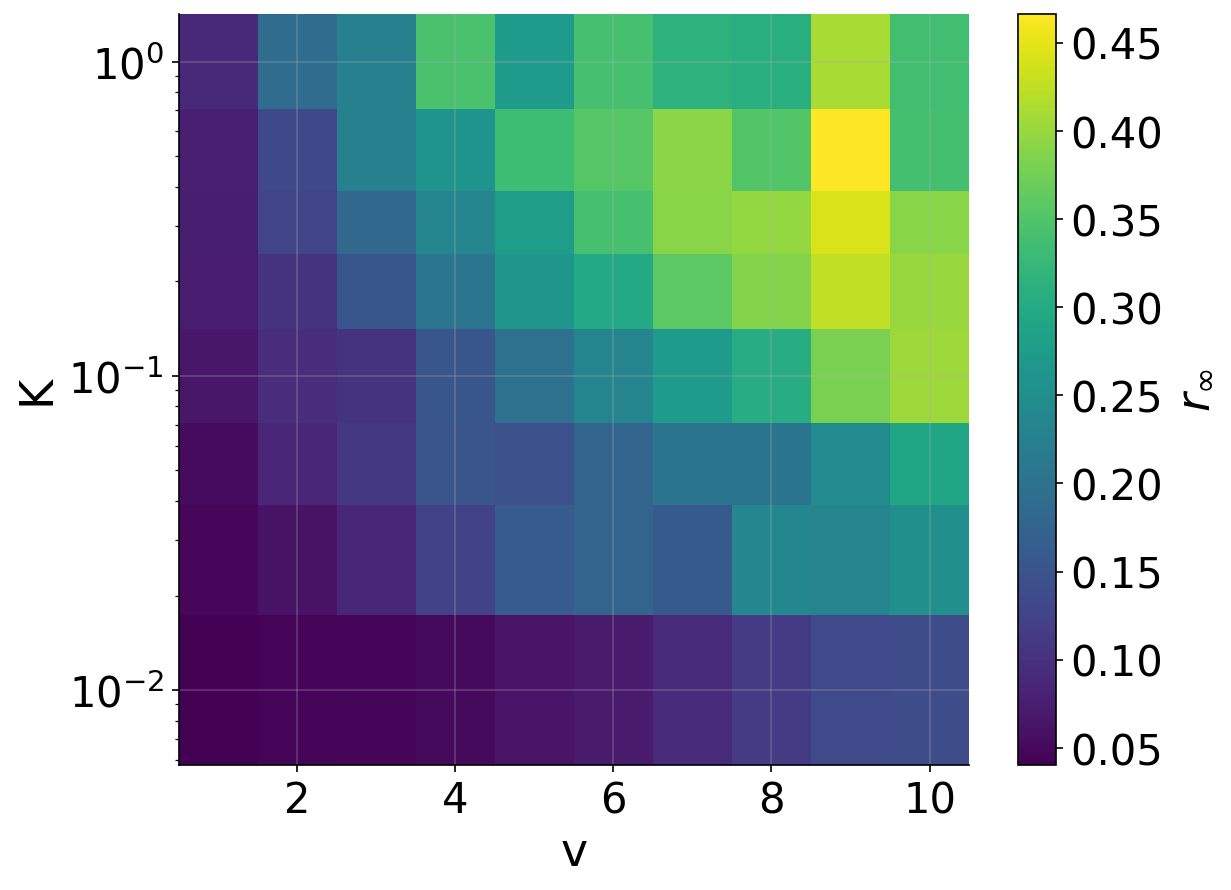
\includegraphics[width=0.8\linewidth]{ring_rvK.png}
  \caption{Diagrama de fases en el plano $(v, K)$; color $= r_\infty$.}
\end{figure}

Ejes $v$ (lineal) y $K$ (log); color $= r_\infty$. La frontera
sincronización/incoherencia se desplaza hacia $K$ más altos cuando $v$ baja: el
``anillo estrecho'' exige más acoplamiento. \textbf{Sin celdas blancas}
($r_\infty$ siempre definido).

\subsection{Mapa de calor $\tau(v, K)$}

\begin{figure}[H]
  \centering
  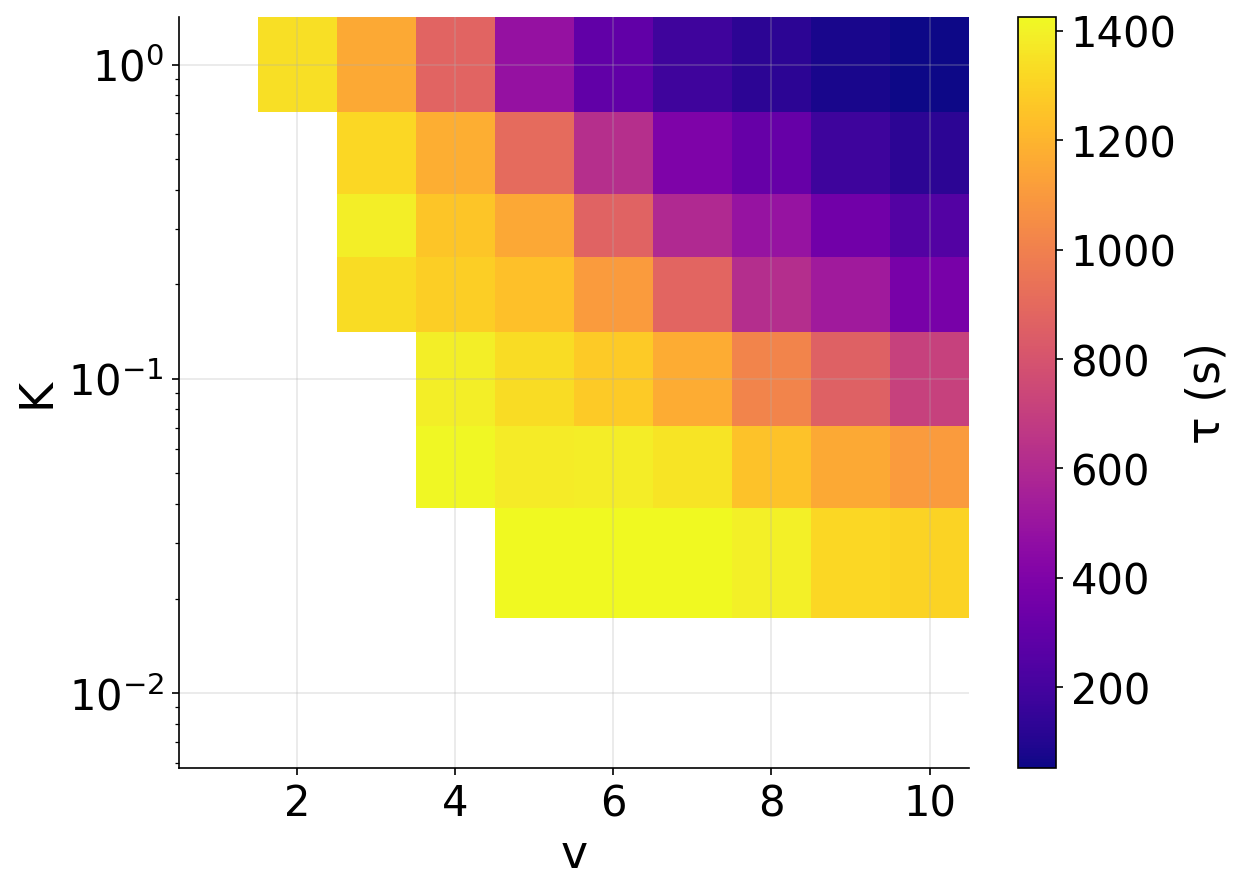
\includegraphics[width=0.8\linewidth]{ring_tauvK.png}
  \caption{Tiempo de sincronización en el plano $(v, K)$; color $= \tau$.}
\end{figure}

Mismo dominio; color plasma $= \tau$. Las \textbf{celdas blancas} son los $(v,K)$
donde menos del 25\% de las 50 realizaciones desarrolla orden ($r_\infty > 0{,}2$,
$< 13$): la región de $v$/$K$ bajos donde el anillo se queda desordenado. La zona
pintada ($\ge 13$ corridas con orden) incluye los estados \emph{parcialmente}
ordenados ($r_\infty$ intermedio), que tienen un transitorio real --- por eso el
mapa muestra muchas más celdas que con el criterio de sincronización plena. Los $\tau$ son mucho mayores que en la completa o la
aleatoria (de ahí el $t_{\text{sim}} = 1500$): el borde de sincronización vive en
$\tau$ de cientos a
$>1000$ s.

\section{Comparativa entre topologías}

\begin{figure}[H]
  \centering
  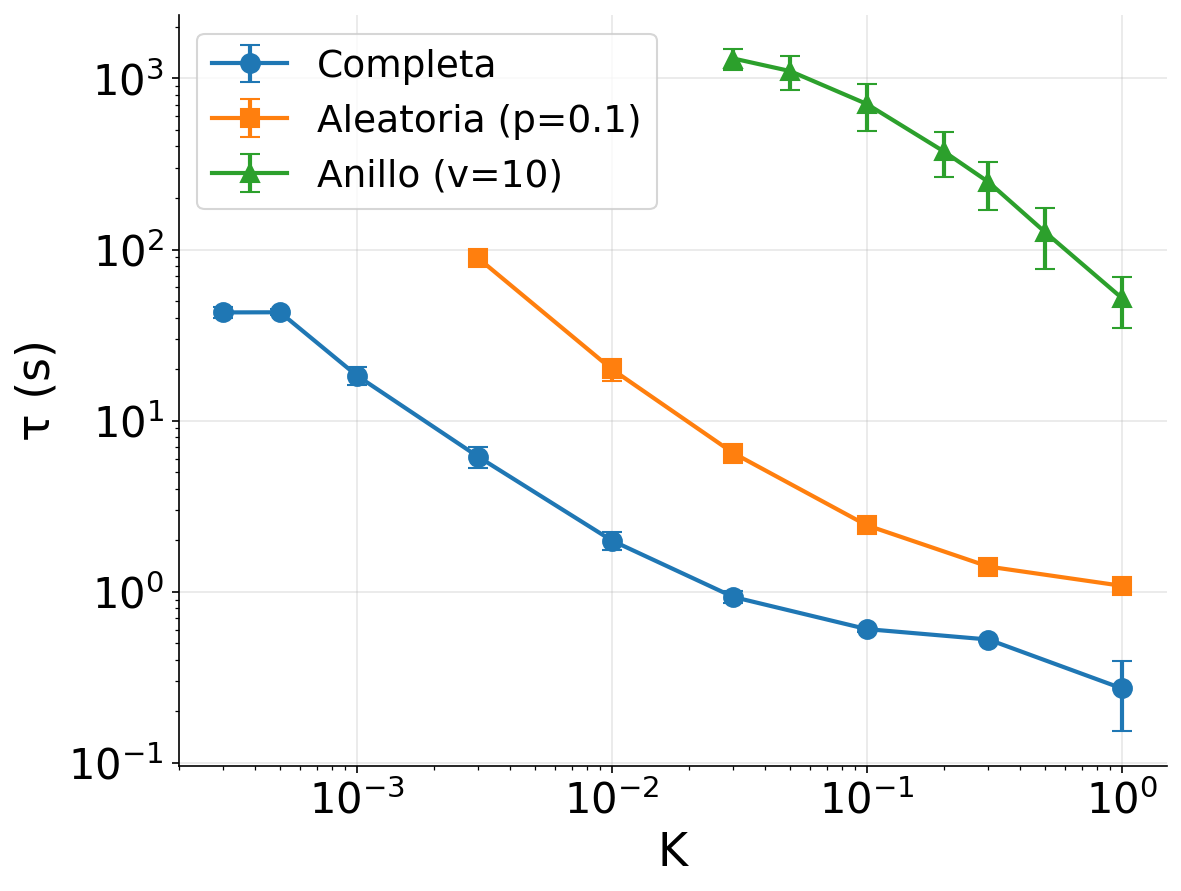
\includegraphics[width=0.8\linewidth]{comparativa_p0.1.png}
  \caption{$\tau(K)$ para las tres topologías, con la red aleatoria a $p = 0{,}1$
  (régimen más conectado dentro del enunciado v2).}
\end{figure}

\begin{itemize}
  \item \textbf{Eje X}: $K$, log.
  \item \textbf{Eje Y}: $\tau$, \textbf{log} (clave: ver abajo).
  \item \textbf{Series}: completa, aleatoria ($p=0{,}1$), anillo ($v=10$).
\end{itemize}

\textbf{Por qué el eje $\tau$ es logarítmico acá} (y lineal en los $\tau(K)$ por
topología): entre topologías, $\tau$ varía muchísimo --- de $\sim 0{,}3$ s
(completa) a $\sim 1000$ s (anillo), casi 4 órdenes de magnitud. En un eje lineal,
las curvas de la completa y la aleatoria (todas $< 50$ s) quedarían aplastadas
contra el cero, indistinguibles al lado del anillo. En log-$\tau$ las tres se ven
separadas y se pueden comparar las pendientes. La completa es la más rápida; la
aleatoria a $p=0{,}1$ ($\langle k\rangle \approx 60$) sincroniza $\sim 1$ orden
más lento pero con la misma pendiente; el anillo ($v=10$, $\langle k\rangle = 20$)
es el más lento, varios órdenes por encima.

\begin{figure}[H]
  \centering
  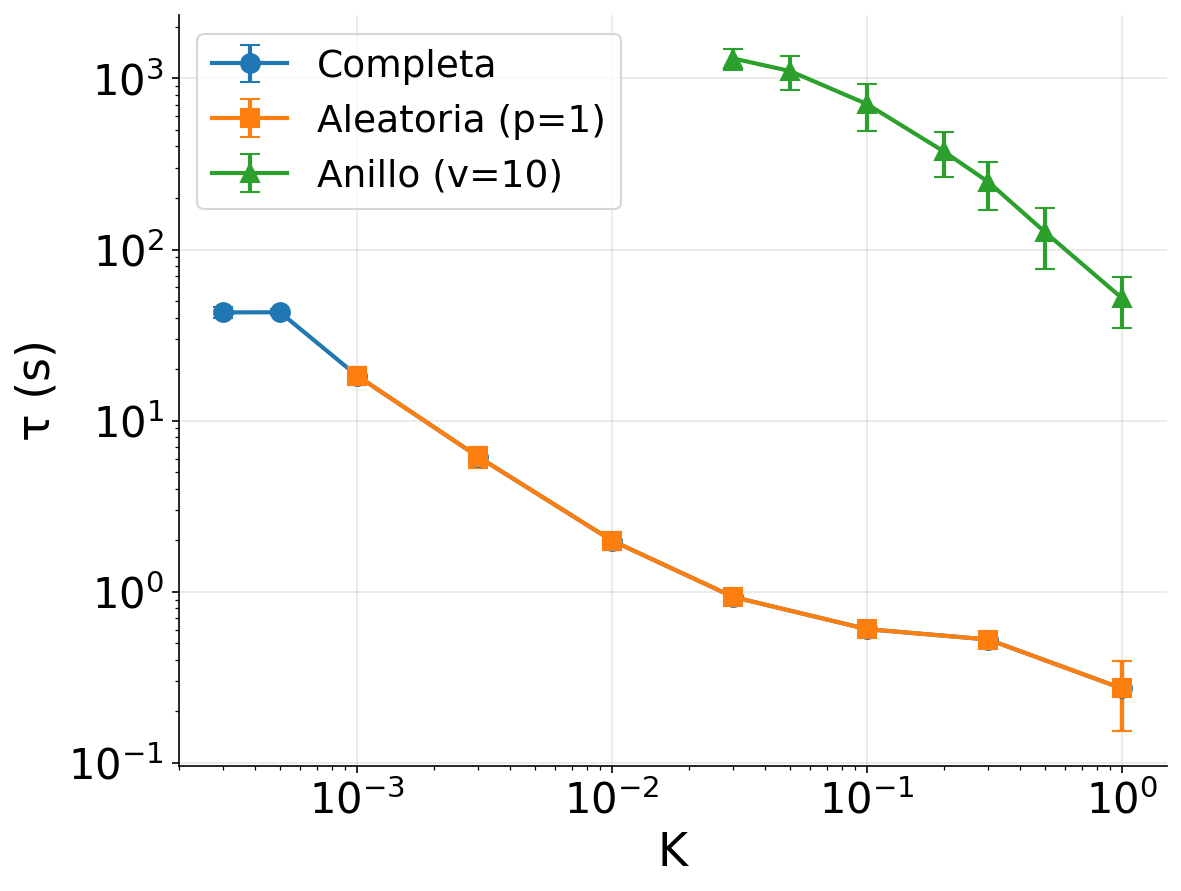
\includegraphics[width=0.8\linewidth]{comparativa.png}
  \caption{Variante con la red aleatoria a $p = 1$ (equivalente a la completa),
  fuera del rango del enunciado v2 pero útil como referencia del régimen
  plenamente conectado.}
\end{figure}

\section{Resumen de elecciones de eje}

\begin{table}[H]
  \centering
  \begin{tabular}{lll}
    \toprule
    \textbf{Eje} & \textbf{Tipo} & \textbf{Motivo} \\
    \midrule
    $t$                    & lineal              & rango acotado y resolución uniforme \\
    $r$                    & lineal $[0, 1{,}05]$ & acotado por definición \\
    $K$                    & log                 & barrido cubre 3--4 órdenes alrededor de $K_c$ \\
    $p$                    & log                 & barrido cubre 4 órdenes de magnitud \\
    $v$                    & lineal              & entero pequeño (1--10), un solo orden \\
    $\tau$ (por topología) & lineal              & rango moderado dentro de una topología \\
    $\tau$ (comparativa)   & log                 & difiere en órdenes de magnitud entre topologías \\
    \bottomrule
  \end{tabular}
\end{table}

\end{document}
